% LTeX: enabled=false
% ============================================================
% TEMPLATE PARA TRABALHO DE CONCLUSÃO DE CURSO
% Universidade Tecnológica Federal do Paraná – UTFPR
% Customização da classe abntex2 para as normas da UTFPR
%
% Motor recomendado : LuaLaTeX
% Bibliografia      : Biber + biblatex-abnt
% ============================================================
% Mudar latex-workshop.view.pdf.viewer nas settings (ctrl + ,). Se estiver em remote access usar browser, se estiver localmente usar tab.

\documentclass[%
%   twoside,          % impressão frente-e-verso
    oneside,          % impressão só frente
    12pt,
    a4paper,
    sumario=abnt-6027-2012,
    brazil,
]{abntex2}

% ── PDF/A ────────────────────────────────────────────────────
% pdfx carrega hyperref e xcolor internamente: NÃO os carregue de
% novo em outro lugar.
% Requer o arquivo main.xmpdata na raiz do projeto (metadados XMP).
\usepackage[a-3u]{pdfx}
% ─────────────────────────────────────────────────────────────

% ── Modo escuro ─────────────────────────────────────────────
% Defina ANTES dos outros \input para que pacotes.tex possa
% ler o booleano ao ser carregado.
\usepackage{etoolbox}
\newbool{darkmode}
\setbool{darkmode}{true}   % true = escuro | false = claro
% ─────────────────────────────────────────────────────────────

% Customizações UTFPR (substitui utfpr-abntex2.cls)
% ============================================================
% configuracoes/utfpr-setup.tex
%
% Customizações da UTFPR sobre a classe abntex2.
% Este arquivo substitui o antigo utfpr-abntex2.cls:
% todas as opções que antes exigiam uma classe própria são
% declaradas aqui, no preâmbulo, mantendo o projeto livre de
% qualquer .cls customizado.
% ============================================================

\RequirePackage{makeidx}    % índice remissivo
\RequirePackage{chngcntr}   % counterwithout / counterwith

% ── Espaçamento ──────────────────────────────────────────────
\frenchspacing

% Sem espaço extra entre parágrafos; indentação de 1,5 cm
\setlength{\parindent}{1.5cm}
\setlength{\parskip}{0pt}

% ── Itens de listas compactos ────────────────────────────────
% (requer enumitem, carregado em pacotes.tex)
\AtBeginDocument{%
    \setlist{noitemsep, topsep=0pt, parsep=0pt, partopsep=0pt}%
}

% ── Equações numeradas sequencialmente (sem prefixo de cap.) ─
\AtBeginDocument{\counterwithout{equation}{chapter}}

% ── Notas de rodapé: numeração contínua ─────────────────────
\AtBeginDocument{\counterwithout{footnote}{chapter}}

% ─────────────────────────────────────────────────────────────
% COMANDOS DE DADOS
% ─────────────────────────────────────────────────────────────

\providecommand{\imprimirdepartamento}{}
\newcommand{\departamento}[1]{\renewcommand{\imprimirdepartamento}{#1}}

\providecommand{\imprimirprograma}{}
\newcommand{\programa}[1]{\renewcommand{\imprimirprograma}{#1}}

\providecommand{\imprimirsubtitulo}{}
\newcommand{\subtitulo}[1]{\renewcommand{\imprimirsubtitulo}{#1}}

\providecommand{\imprimirinstOrientador}{}
\newcommand{\instOrientador}[1]{\renewcommand{\imprimirinstOrientador}{#1}}

\providecommand{\imprimirinstCoorientador}{}
\newcommand{\instCoorientador}[1]{\renewcommand{\imprimirinstCoorientador}{#1}}

\providecommand{\imprimirprojeto}{}
\newcommand{\projeto}[1]{\renewcommand{\imprimirprojeto}{#1}}

\providecommand{\imprimirtituloAcademico}{}
\newcommand{\tituloAcademico}[1]{\renewcommand{\imprimirtituloAcademico}{#1}}

\providecommand{\imprimirautorcitacao}{}
\newcommand{\autorcitacao}[1]{\renewcommand{\imprimirautorcitacao}{#1}}

\providecommand{\imprimirtitleabstract}{}
\newcommand{\titleabstract}[1]{\renewcommand{\imprimirtitleabstract}{#1}}

\newcommand{\imprimirareaconcentracaoRotulo}{Área de concentração: }
\providecommand{\imprimirareaconcentracao}{}
\newcommand{\areaconcentracao}[1]{\renewcommand{\imprimirareaconcentracao}{#1}}

\newcommand{\imprimirlinhapesquisaRotulo}{Linha de pesquisa: }
\providecommand{\imprimirlinhapesquisa}{}
\newcommand{\linhapesquisa}[1]{\renewcommand{\imprimirlinhapesquisa}{#1}}

\providecommand{\imprimirtextopadraofolhadeaprovacao}{}
\newcommand{\textopadraofolhadeaprovacao}[1]{%
    \renewcommand{\imprimirtextopadraofolhadeaprovacao}{#1}}

% \logoinstituicao{<escala>}{<caminho>}
\providecommand{\imprimirlogoinstituicao}{}
\newcommand{\logoinstituicao}[2]{%
    \renewcommand{\imprimirlogoinstituicao}{%
        \includegraphics[width={#1}\textwidth]{#2}}}

% ─────────────────────────────────────────────────────────────
% ESTILO DE PÁGINAS
% ─────────────────────────────────────────────────────────────

\renewcommand{\pretextual}{%
    \pagenumbering{gobble}
    \aliaspagestyle{chapter}{empty}
    \pagestyle{empty}
    \aliaspagestyle{cleared}{empty}
    \aliaspagestyle{part}{empty}
}

\renewcommand{\textual}{%
    \pagenumbering{arabic}
    \pagestyle{abntheadings}
    \aliaspagestyle{chapter}{abntchapfirst}
    \nouppercaseheads
    \bookmarksetup{startatroot}
}

\renewcommand{\postextual}{%
    \chapterstyle{abnt}
    \phantompart
}

% ─────────────────────────────────────────────────────────────
% FONTES DOS TÍTULOS (norma ABNT/UTFPR)
% ─────────────────────────────────────────────────────────────

\renewcommand{\ABNTEXchapterfont}{\normalfont\bfseries}
\renewcommand{\ABNTEXchapterfontsize}{\normalsize}

\renewcommand{\ABNTEXpartfont}{\normalfont}
\renewcommand{\ABNTEXpartfontsize}{\ABNTEXchapterfontsize}

\renewcommand{\ABNTEXsectionfont}{\normalfont}
\renewcommand{\ABNTEXsectionfontsize}{\normalsize}

\renewcommand{\ABNTEXsubsectionfont}{\normalfont}
\renewcommand{\ABNTEXsubsectionfontsize}{\normalsize}

\renewcommand{\ABNTEXsubsubsectionfont}{\normalfont}
\renewcommand{\ABNTEXsubsubsectionfontsize}{\normalsize}

\renewcommand{\ABNTEXsubsubsubsectionfont}{\normalfont}
\renewcommand{\ABNTEXsubsubsubsectionfontsize}{\normalsize}

% ─────────────────────────────────────────────────────────────
% SUMÁRIO
% ─────────────────────────────────────────────────────────────

\makeatletter
\renewcommand{\cftchapteraftersnum}{\quad}
\setlength{\cftbeforechapterskip}{1.0em \@plus\p@}
\makeatother

% Nível 1   — NEGRITO E MAIÚSCULAS (abntex2 já aplica \MakeUppercase nas entradas de capítulo)
\renewcommand{\cftchapterfont}{\bfseries}
% Nível 1.1 — Negrito, Misto
\renewcommand{\cftsectionfont}{\bfseries}
% Nível 1.1.1 — Itálico, Misto
\renewcommand{\cftsubsectionfont}{\normalfont\itshape}
% Nível 1.1.1.1 — Itálico + Sublinhado, Misto  (requer ulem, carregado em pacotes.tex)
\renewcommand{\cftsubsubsectionfont}{\normalfont\itshape}
\makeatletter
\let\UTFPR@old@l@subsubsection\l@subsubsection
\renewcommand*{\l@subsubsection}[2]{%
  \UTFPR@old@l@subsubsection{\uline{#1}}{#2}%
}
\makeatother

% ─────────────────────────────────────────────────────────────
% LISTAS (nomes e rótulos)
% ─────────────────────────────────────────────────────────────

\addto\captionsbrazil{%
    \renewcommand{\listadesiglasname}{LISTA DE ABREVIATURAS E SIGLAS}
    \renewcommand{\listadesimbolosname}{LISTA DE S\'IMBOLOS}
    \renewcommand{\listfigurename}{LISTA DE FIGURAS}
    \renewcommand{\listtablename}{LISTA DE TABELAS}
    \renewcommand{\indexname}{\'INDICE REMISSIVO}
    % autoref
    \renewcommand{\pageautorefname}{p\'agina}
    \renewcommand{\sectionautorefname}{Se\c{c}\~ao}
    \renewcommand{\subsectionautorefname}{Subse\c{c}\~ao}
    \renewcommand{\subsubsectionautorefname}{Subsubse\c{c}\~ao}
    \renewcommand{\paragraphautorefname}{Subse\c{c}\~ao}
}

% Lista de Quadros
\newcommand{\listofquadrosname}{Lista de Quadros}
\newcommand{\quadroname}{Quadro}
\newfloat[chapter]{quadro}{loq}{\quadroname}
\newlistof{listofquadros}{loq}{\listofquadrosname}
\newlistentry{quadro}{loq}{0}
\counterwithout{quadro}{chapter}
\renewcommand{\cftquadroname}{\quadroname\space}
\renewcommand*{\cftquadroaftersnum}{\hfill--\hfill}

% ─────────────────────────────────────────────────────────────
% OBJETOS FLUTUANTES — fonte e nota
% ─────────────────────────────────────────────────────────────

\renewcommand{\fonte}[1]{%
    \begin{SingleSpacing}\par\end{SingleSpacing}
    \centering\small{\textbf{Fonte:} #1}%
}

\renewcommand{\nota}[1]{%
    \begin{SingleSpacing}\par\end{SingleSpacing}
    \begin{tabular}{l p{.85\textwidth}}%
        Nota: & #1
    \end{tabular}%
}

% ─────────────────────────────────────────────────────────────
% CAPA
% ─────────────────────────────────────────────────────────────

\makeatletter
\renewcommand{\imprimircapa}{%
    \begin{capa}
        \begin{center}
            \begin{SingleSpacing}
                \large\MakeUppercase{\imprimirinstituicao}\\
                \abntex@ifnotempty{\imprimirdepartamento}{%
                    \MakeUppercase{\imprimirdepartamento}\\
                }%
                \large\MakeUppercase{\imprimirprograma}\\
            \end{SingleSpacing}
        \end{center}
        \vspace{60pt}
        \begin{center}
            \large\MakeUppercase{\imprimirautor}\\
        \end{center}
        \vspace{120pt}
        \begin{center}
            \ABNTEXchapterfont\large\MakeUppercase{\imprimirtitulo}
            \abntex@ifnotempty{\imprimirsubtitulo}{%
                {\ABNTEXchapterfont: }{\large{\imprimirsubtitulo}}%
            }
        \end{center}
        \vspace{120pt}
        \begin{center}
            \large\MakeUppercase{\imprimirprojeto}
        \end{center}
        \vfill
        \begin{center}
            \begin{SingleSpacing}
                \large\MakeUppercase{\imprimirlocal}\\
                \large\MakeUppercase{\imprimirdata}
            \end{SingleSpacing}
        \end{center}
    \end{capa}
}
\makeatother

% ─────────────────────────────────────────────────────────────
% FOLHA DE ROSTO
% ─────────────────────────────────────────────────────────────

\makeatletter
\renewcommand{\folhaderostocontent}{%
    \setcounter{page}{2}
    \begin{center}
        \large\MakeUppercase{\imprimirautor}\\
    \end{center}

    \vspace*{96pt}

    \begin{center}
        \ABNTEXchapterfont\large\MakeUppercase{\imprimirtitulo}
        \abntex@ifnotempty{\imprimirsubtitulo}{%
            {\ABNTEXchapterfont: }{\large{\imprimirsubtitulo}}%
        }
    \end{center}

    \vspace*{60pt}

    \abntex@ifnotempty{\imprimirpreambulo}{%
        \SingleSpacing
        \begin{tabular}{p{.25\textwidth}p{.13\textwidth}p{.44\textwidth}}
             & \multicolumn{2}{p{.6\textwidth}}{                                   %
            \small\hyphenpenalty=10000{\imprimirpreambulo}}                        \\ & & \\
            \abntex@ifnotempty{\imprimirareaconcentracao}{%
             & \multicolumn{2}{p{.6\textwidth}}{                                   %
            \small\hyphenpenalty=10000{%
            \imprimirareaconcentracaoRotulo\imprimirareaconcentracao}%
            }                                                                      \\ & & \\
            }%
            \abntex@ifnotempty{\imprimirlinhapesquisa}{%
             & \multicolumn{2}{p{.6\textwidth}}{                                   %
            \small\hyphenpenalty=10000{%
            \imprimirlinhapesquisaRotulo\imprimirlinhapesquisa}%
            }                                                                      \\ & & \\
            }%
            \abntex@ifnotempty{\imprimirorientador}{%
             & \small\imprimirorientadorRotulo   & \imprimirorientador             \\
             &                                   & \small\imprimirinstOrientador   \\ & & \\
            }%
            \abntex@ifnotempty{\imprimircoorientador}{%
             & \small\imprimircoorientadorRotulo & \imprimircoorientador           \\
             &                                   & \small\imprimirinstCoorientador
            }%
        \end{tabular}
    }

    \vspace*{\fill}

    \begin{center}
        \begin{SingleSpacing}
            \large\MakeUppercase{\imprimirlocal}\\
            \large\MakeUppercase{\imprimirdata}
        \end{SingleSpacing}
    \end{center}
}
\makeatother

% ─────────────────────────────────────────────────────────────
% FOLHA DE APROVAÇÃO
% ─────────────────────────────────────────────────────────────

\makeatletter
\newcommand{\imprimirfolhadeaprovacao}{%
    \begin{folhadeaprovacao}
        \vspace*{\fill}
        \begin{tabular}{p{.45\textwidth}p{.45\textwidth}}
             & \imprimirtextopadraofolhadeaprovacao \\
        \end{tabular}
        \vspace*{\fill}
    \end{folhadeaprovacao}
}
\makeatother

% ─────────────────────────────────────────────────────────────
% DEDICATÓRIA
% ─────────────────────────────────────────────────────────────

\renewenvironment{dedicatoria}[1][]{%
    \ifthenelse{\equal{#1}{}}{%
        \PRIVATEbookmarkthis{\dedicatorianame}%
    }{\pretextualchapter{#1}}%
    \vspace*{\fill}
    \begin{flushright}
        \begin{minipage}{.5\textwidth}
            \begin{SingleSpacing}
                \setlength\parindent{0pt}
                \setlength\parskip{12pt}
                }{%
            \end{SingleSpacing}
        \end{minipage}
    \end{flushright}
}

% ─────────────────────────────────────────────────────────────
% EPÍGRAFE
% ─────────────────────────────────────────────────────────────

\renewenvironment{epigrafe}[1][]{%
    \ifthenelse{\equal{#1}{}}{%
        \PRIVATEbookmarkthis{\epigraphname}%
    }{\pretextualchapter{#1}}%
    \vspace*{\fill}
    \begin{flushright}
        \begin{minipage}{.5\textwidth}
            \begin{SingleSpacing}
                \setlength\parindent{0pt}
                \setlength\parskip{12pt}
                }{%
            \end{SingleSpacing}
        \end{minipage}
    \end{flushright}
}


% Pacotes
\input{configuracoes/pacotes}

% Configurações do PDF/hyperref
% LTeX: enabled=false
% ============================================================
% configuracoes/configuracoes-pdf.tex
%
% Configurações finais do PDF (hyperref, índice, hifenização).
% Carregado APÓS pacotes.tex (hyperref já foi carregado lá).
% ============================================================

% ── hyperref ─────────────────────────────────────────────────
\makeatletter
\hypersetup{%
    portuguese,
    hidelinks,          % sem cor e sem caixa; o negrito abaixo diferencia os links
    %    colorlinks  = true,
    breaklinks  = true,
    %    linkcolor   = \ifbool{darkmode}{DarkModeLink}{LightModeLink},
    %    citecolor   = \ifbool{darkmode}{DarkModeLink}{LightModeLink},
    %    filecolor   = \ifbool{darkmode}{DarkModeLink}{LightModeLink},
    %    urlcolor    = \ifbool{darkmode}{DarkModeLink}{LightModeLink},
    pdftitle    = {\@title},
    pdfauthor   = {\@author},
    pdfkeywords = {abnt, latex, abntex, abntex2, utfpr},
}
\makeatother

% ── Links em negrito (substituição de \hyperref colorido) ────
% Redefine o hook interno do hyperref para injetar \bfseries
% no início de cada link. Afeta \ref, \cite, \url, \href, etc.
\makeatletter
\let\UTFPR@hyper@linkstart\hyper@linkstart
\renewcommand{\hyper@linkstart}[2]{%
    \UTFPR@hyper@linkstart{#1}{#2}\bfseries
}
\makeatother

% ── Rótulos de \autoref ──────────────────────────────────────
\renewcommand{\algorithmautorefname}{Algoritmo}
\def\equationautorefname~#1\null{Equa\c{c}\~ao~(#1)\null}

% ── Índice remissivo ─────────────────────────────────────────
\makeindex

% ── Hifenização de palavras não reconhecidas ─────────────────
\hyphenation{%
    qua-dros-cha-ve
    Kat-sa-gge-los
}


% ── Dados e capa ─────────────────────────────────────────────
%!TEX root = ../../main.tex
% ============================================================
% estrutura/pre-textuais/capa.tex
%
% DADOS DO TRABALHO — edite esta seção antes de tudo
% ============================================================

% ── Título e subtítulo ───────────────────────────────────────
\titulo{Infinitos de Cantor}
\subtitulo{Cardinalidade, Dimensão e a Estrutura dos Números Ordinais}

% ── Título em inglês (usado no Abstract) ────────────────────
\titleabstract{Cantor's Infinities: Cardinality, Dimension, and the Structure of Ordinal Numbers}

% ── Autor ────────────────────────────────────────────────────
\autor{Eduardo Furlan}
\autorcitacao{FURLAN, Eduardo}  % Sobrenome em maiúsculo

% ── Local e ano ──────────────────────────────────────────────
\local{Pato Branco}
\data{2026}

% ── Natureza do trabalho ─────────────────────────────────────
% Opções: Trabalho de Conclusão de Curso | Dissertação | Tese
%         Projeto de Qualificação
\projeto{Trabalho de Conclusão de Curso}

% ── Título acadêmico ─────────────────────────────────────────
% Opções: Bacharel | Tecnólogo | Licenciado | Mestre | Doutor
\tituloAcademico{Licenciado}

% ── Instituição ──────────────────────────────────────────────
% Se for TCC, coloque o nome do curso em \programa{}
% \logoinstituicao{<escala>}{<caminho/nome do arquivo>}
\instituicao{\textbf{Universidade Tecnológica Federal do Paraná}}
\departamento{\textbf{DAMAT}}
\programa{\textbf{Curso de Licenciatura em Matemática}}
\logoinstituicao{0.2}{../../dados/figuras/logo-instituicao.png}

% ── Área de concentração / linha de pesquisa ─────────────────
% Deixe vazios para TCC de graduação
\areaconcentracao{}
\linhapesquisa{}

% ── Orientador(a) ────────────────────────────────────────────
\orientador{Prof. Dr. Ivan Italo Gonzales Gargate}
% \orientador[Orientadora:]{Profa. Dra. Nome da Orientadora}
\instOrientador{Universidade Tecnológica Federal do Paraná}

% ── Coorientador(a) — descomente se houver ──────────────────
% \coorientador{Prof. Dr. Nome do Coorientador}
% \instCoorientador{Instituição do Coorientador}

%!TEX root = ../../main.tex
% ============================================================
% estrutura/pre-textuais/folha-rosto.tex
%
% Define o preâmbulo (natureza do trabalho) que aparece na
% Folha de Rosto. Descomente apenas a linha correspondente
% ao tipo do seu trabalho.
% ============================================================

% Trabalho de Conclusão de Curso (graduação)
\preambulo{{\imprimirprojeto} apresentado no {\imprimirprograma} da {\imprimirinstituicao}, como requisito parcial para a obtenção do título de {\imprimirtituloAcademico}.}

% Dissertação de Mestrado
% \preambulo{{\imprimirprojeto} apresentada ao Programa de \mbox{Pós-graduação} da {\imprimirinstituicao}, como requisito parcial para obtenção do título de {\imprimirtituloAcademico}.}

% Tese de Doutorado
% \preambulo{{\imprimirprojeto} apresentada ao Programa de \mbox{Pós-graduação} da {\imprimirinstituicao}, como requisito parcial para a obtenção do título de {\imprimirtituloAcademico}.}

% Projeto de Qualificação (mestrado ou doutorado)
% \preambulo{{\imprimirprojeto} apresentado ao Programa de \mbox{Pós-graduação} da {\imprimirinstituicao}, como requisito parcial para a obtenção do título de {\imprimirtituloAcademico}.}

% ─────────────────────────────────────────────────────────────

\begin{document}

% ── Elementos pré-textuais ───────────────────────────────────
\pretextual
\imprimircapa
\imprimirfolhaderosto{}

\include{estrutura/pre-textuais/dedicatoria}
\include{estrutura/pre-textuais/agradecimentos}
\include{estrutura/pre-textuais/epigrafe}
\include{estrutura/pre-textuais/resumo}
\include{estrutura/pre-textuais/abstract}

\include{estrutura/pre-textuais/listas/listas-ilustracoes/lista-figuras}
\include{estrutura/pre-textuais/listas/listas-ilustracoes/lista-quadros}
\include{estrutura/pre-textuais/listas/lista-tabelas}
\pretextualchapter{LISTA DE ENUNCIADOS}
\pdfbookmark[0]{Lista de Teoremas}{loe}

\begingroup
% Ajuste Visual: Transforma títulos de capítulos em seções
\let\chapter\section
\renewcommand{\addcontentsline}[3]{}

% Formata o nome opcional como " - nome" em vez de " (nome)"
\renewcommand{\thmtformatoptarg}[1]{ - #1}

% --- AXIOMAS ---
\renewcommand{\listtheoremname}{Axiomas}
\listoftheorems[swapnumber, ignoreall, show={axioma}]

% --- DEFINIÇÕES ---
\renewcommand{\listtheoremname}{Definições}
\listoftheorems[swapnumber, ignoreall, show={definicao}]

% --- TEOREMAS ---
\renewcommand{\listtheoremname}{Teoremas}
\listoftheorems[swapnumber, ignoreall, show={teorema}]

% --- COROLÁRIOS ---
\renewcommand{\listtheoremname}{Corolários}
\listoftheorems[swapnumber, ignoreall, show={corolario}]

% --- LEMAS ---
\renewcommand{\listtheoremname}{Lemas}
\listoftheorems[swapnumber, ignoreall, show={lema}]

% --- PROPOSIÇÕES ---
\renewcommand{\listtheoremname}{Proposições}
\listoftheorems[swapnumber, ignoreall, show={proposicao}]

\endgroup
\cleardoublepage

\include{estrutura/pre-textuais/listas/lista-siglas}
\include{estrutura/pre-textuais/listas/lista-simbolos}
% \include{estrutura/pre-textuais/listas/listas-diversas/lista-algoritmos}

\include{estrutura/pre-textuais/sumario}

% ── Elementos textuais ───────────────────────────────────────
\textual

\include{estrutura/textuais/introducao}

\include{estrutura/textuais/desenvolvimento/fundamentos_teoria_conjuntos}

\include{estrutura/textuais/desenvolvimento/cardinalidade}

\include{estrutura/textuais/desenvolvimento/infinitos}

\include{estrutura/textuais/desenvolvimento/hipotese_continuo}

\include{estrutura/textuais/desenvolvimento/cardinais_dimensao}

\include{estrutura/textuais/desenvolvimento/ordinais}

\include{estrutura/textuais/desenvolvimento/escolha}

\include{estrutura/textuais/desenvolvimento/metodologia}

% \include{estrutura/textuais/desenvolvimento/resultados}

% %!TEX root = ../../../main.tex
% ============================================================
% estrutura/textuais/desenvolvimento/orientacoes.tex
%
% Capítulo de orientações de uso do template.
% Remova o \include correspondente em main.tex quando não
% for mais necessário.
% ============================================================

% ── Ilustrações ──────────────────────────────────────────────
\chapter{SOBRE AS ILUSTRAÇÕES}
\label{chap:apSobreIlust}

A seguir exemplifica-se como inserir ilustrações no corpo do trabalho.
As ilustrações são indexadas automaticamente em suas respectivas listas.
Referências cruzadas são obtidas através dos comandos \verb|\label{}| e
\verb|\autoref{}|: por exemplo, \autoref{fig:figura-exemplo1}.

% ── Figuras ──────────────────────────────────────────────────
\chapter{FIGURAS}
\label{chap:figuras}

\begin{figure}[!htb]
    \centering
    \caption{Exemplo de Figura}
    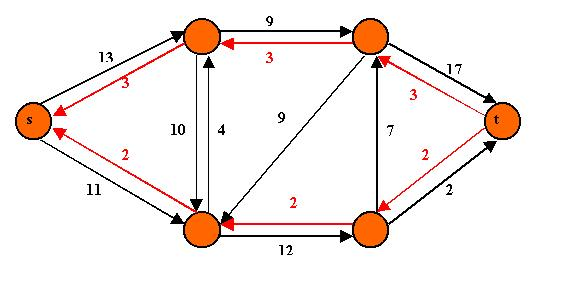
\includegraphics[width=0.5\textwidth]{./dados/figuras/figura1}
    \fonte{\textcite{chave}}
    \label{fig:figura-exemplo1}
\end{figure}

% ── Quadros e Tabelas ────────────────────────────────────────
\chapter{QUADROS E TABELAS}
\label{chap:tabelas}

Exemplo de como inserir o \autoref{qua:quadro-exemplo1} e a \autoref{tab:tabela-exemplo1}. Ambos aparecem automaticamente nas suas respectivas listas. Para saber mais informações sobre a construção de tabelas no \LaTeX{} consulte literatura especializada \cite{Mittelbach2004}.

Ambos os elementos (Quadros e Tabelas) devem ser criados em arquivos separados para facilitar manutenção e armazenados no diretório de ``/dados''.

\input{./dados/quadros/quadro1}

A diferença entre quadro e tabela está no fato que um quadro é formado por linhas horizontais e verticais. Deve ser utilizado quando o conteúdo é majoritariamente não-numérico. O número do quadro e o título vem acima do quadro, e a fonte, deve vir abaixo. E Uma tabela é formada apenas por linhas verticais. Deve ser utilizada quando o conteúdo é majoritariamente numérico. O número da tabela e o título vem acima da tabela, e a fonte, deve vir abaixo, tal como no quadro.

\input{./dados/tabelas/tabela1}

% ── Equações ─────────────────────────────────────────────────
\chapter{EQUAÇÕES}
\label{chap:equacoes}

Exemplo de como inserir a \autoref{eq:equacao-exemplo1} e a Eq. \ref{eq:equacao-exemplo2} no corpo do texto \footnote{Deve-se atentar ao fato de a formatação das equações ficar muito boa esteticamente.}. Observe que foram utilizadas duas formas distintas para referenciar as equações.

\begin{equation}
    X(s) = \int\limits_{t=-\infty}^{\infty} x(t)\,\mathrm{e}^{-st}\,\mathrm{d}t
    \label{eq:equacao-exemplo1}
\end{equation}

\begin{equation}
    F(u, v) = \sum_{m = 0}^{M - 1} \sum_{n = 0}^{N - 1} f(m, n) \exp \left[ -j 2 \pi \left( \frac{u m}{M} + \frac{v n}{N} \right) \right]
    \label{eq:equacao-exemplo2}
\end{equation}

% ── Algoritmos ───────────────────────────────────────────────
\chapter{ALGORITMOS}
\label{chap:algoritmos}

Exemplo de como inserir um algoritmo. Para inserção de algoritmos utiliza-se o pacote {\ttfamily algorithm2e} que já está devidamente configurado dentro do template.

Os algoritmos devem ser criados em arquivos separados para facilitar manutenção e armazenados no diretório de ``/dados''.\\
\\

\input{./dados/algoritmos/algoritmo1}

% ── Listas ───────────────────────────────────────────────
\chapter{SOBRE AS LISTAS}
\label{chap:apSobreLista}

Para construir listas de ``\textit{bullets}''{} ou listas enumeradas, inclusive listas aninhadas, é utilizado o pacote \verb|paralist|.

Exemplo de duas listas não numeradas aninhadas, utilizando o comando \verb|\itemize|. Observe a indentação, bem como a mudança automática do tipo de ``\textit{bullet}''{} nas listas aninhadas.

\begin{itemize}
    \item item não numerado 1
    \item item não numerado 2
          \begin{itemize}
              \item subitem não numerado 1
              \item subitem não numerado 2
              \item subitem não numerado 3
          \end{itemize}
    \item item não numerado 3
\end{itemize}

Exemplo de duas listas numeradas aninhadas, utilizando o comando \verb|\enumerate|. Observe a numeração progressiva e indentação das listas aninhadas.

\begin{enumerate}
    \item item numerado 1
    \item item numerado 2
          \begin{enumerate}
              \item subitem numerado 1
              \item subitem numerado 2
              \item subitem numerado 3
          \end{enumerate}
    \item item numerado 3
\end{enumerate}

% ── Uso do biblatex ──────────────────────────────────────────
\chapter{REFERÊNCIAS BIBLIOGRÁFICAS}
\label{chap:referencias}

Este template usa \textbf{biblatex} + \textbf{biber}. Comandos:

\begin{itemize}
    \item \verb|\parencite{chave}| → \parencite{chave}
    \item \verb|\textcite{chave}|  → \textcite{chave}
    \item \verb|\citeyear{chave}|  → \citeyear{chave}
\end{itemize}

\chapter{CITAÇÕES DIRETAS}
\label{chap:citacoesLiterais}

É a transcrição ou cópia de um parágrafo, de uma frase, de parte dela ou de uma expressão, usando exatamente as mesmas palavras adotadas pelo autor do trabalho consultado.

Quanto à chamada da referência, ela pode ser feita de qualquer das duas maneiras já mencionadas nas citações indiretas, conforme o nome do(s) autor(es) façam parte do texto ou não. Há duas maneiras distintas de se fazer uma citação direta, conforme o trecho citado seja longo ou curto.

Quando o trecho citado é longo (4 ou mais linhas) deve-se usar um parágrafo específico para a citação, na forma de um texto recuado (4 cm da margem esquerda), com tamanho de letra menor e espaçamento entrelinhas simples. Exemplo de citação longa:
\\\begin{citacao}
    Desse modo, opera-se uma ruptura decisiva entre a reflexividade filosófica, isto é a possibilidade do sujeito de pensar e de refletir, e a objetividade científica. Encontramo-nos num ponto em que o conhecimento científico está sem consciência. Sem consciência moral, sem consciência reflexiva e também subjetiva. Cada vez mais o desenvolvimento extraordinário do conhecimento científico vai tornar menos praticável a própria possibilidade de reflexão do sujeito sobre a sua pesquisa \cite[p.~28]{Silva2000}.
\end{citacao}

Para fazer a citação longa deve-se utilizar os seguintes comandos:
\begin{verbatim}
\begin{citacao}
<texto da citacao>
\end{citacao}
\end{verbatim}

No exemplo acima, para a chamada da referência o comando \verb|\cite[p.~28]{Silva2000}| foi utilizado, visto que os nomes dos autores não são parte do trecho citado. É necessário também indicar o número da página da obra citada que contém o trecho citado.

Quando o trecho citado é curto (3 ou menos linhas) ele deve inserido diretamente no texto entre aspas. Exemplos de citação curta:\\
\\A epistemologia baseada na biologia parte do princípio de que ``assumo que não posso fazer referência a entidades independentes de mim para construir meu explicar'' \cite[p.~35]{Maturana2003}.\\
\\A epistemologia baseada na biologia de \textcite[p.~35]{Maturana2003} parte do princípio de que ``assumo que não posso fazer referência a entidades independentes de mim para construir meu explicar''.


Compilação: \texttt{latexmk -lualatex main}

\chapter{SOBRE AS REFERÊNCIAS BIBLIOGRÁFICAS}
\label{chap:apSobreRefer}

A bibliografia é feita no padrão \textsc{Bib}\TeX{}. As referências são colocadas em um arquivo separado. Neste template as referências são armazenadas no arquivo ``base-referencias.bib''.

Existem diversas categorias documentos e materiais componentes da bibliografia. A classe abn\TeX{} define as seguintes categorias (entradas):

\begin{verbatim}
@book
@inbook
@article
@phdthesis
@mastersthesis
@monography
@techreport
@manual
@proceedings
@inproceedings
@journalpart
@booklet
@patent
@unpublished
@misc
\end{verbatim}

Cada categoria (entrada) é formatada pelo pacote \textcite{abnTeX22014d} de uma forma específica. Algumas entradas foram introduzidas especificamente para atender à norma \textcite{NBR6023:2002}, são elas: \verb|@monography|, \verb|@journalpart|,\verb|@patent|. As demais entradas são padrão \textsc{Bib}\TeX{}. Para maiores detalhes, refira-se a \textcite{abnTeX22014d}, \textcite{abnTeX22014b}, \textcite{abnTeX22014c}.

% NOTAS DE RODAPÉ--------------------------------------------------------------------------
\chapter{NOTAS DE RODAPÉ}
\label{chap:notasRodape}

As notas de rodapé pode ser classificadas em duas categorias: notas explicativas\footnote{é o tipo mais comum de notas que destacam, explicam e/ou complementam o que foi dito no corpo do texto, como esta nota de rodapé, por exemplo.} e notas de referências. A notas de referências, como o próprio nome ja indica, são utilizadas para colocar referências e/ou chamadas de referências sob certas condições.
 % Capítulo com Orientações de uso do Template

% \include{estrutura/textuais/conclusao}

% ── Elementos pós-textuais ───────────────────────────────────
\postextual

%!TEX root = ../../main.tex
% ============================================================
% estrutura/pos-textuais/referencias.tex
%
% Impressão das referências bibliográficas.
% Com biblatex não há mais \bibliography{} nem \bibliographystyle{}.
% ============================================================
\nocite{*}

\printbibliography[%
  title={REFER\^ENCIAS},
  heading=bibintoc,
  category=cited
]

\newpage
\printbibliography[
  notcategory=cited,
  title={REFER\^ENCIAS AINDA NÃO CITADAS}
]
%!TEX root = main.tex
% APÊNDICES--------------------------------------------------------------------

\begin{apendicesenv}
    \partapendices

    \chapter{Paradoxos de Tamanho e Contagem}
\label{chap:apendiceTamanhoContagem}

Os paradoxos reunidos neste apêndice formam uma narrativa histórica
que parte da Grécia Antiga e culmina na teoria cantoriana, cada um deles revelou uma insuficiência no entendimento vigente do infinito e motivou avanços fundamentais na matemática.

\section{Os Paradoxos de Zenão (c. 450 a.C.)}

Apresentar Aquiles e a tartaruga, a flecha em repouso, e a dicotomia. Mostrar que a inquietação com somas infinitas e divisibilidade infinita é anterior à matemática formal em mais de dois milênios.


\section{O Paradoxo de Galileu (1638)}

Apresentar a bijeção \(n \to n^2\) entre os naturais e os quadrados perfeitos. Contextualizar como o primeiro registro moderno de estranheza com bijeções em conjuntos infinitos. Conectar com a Definição de conjunto infinito do Capítulo 3.


\section{O Hotel de Hilbert (1924)}

Apresentar o experimento mental: hotel com infinitos quartos, todos ocupados, que ainda assim acomoda novos hóspedes inclusive infinitos deles. Conectar com a aritmética cardinal do Capítulo 6 (\(ℵ_0 + ℵ_0 = ℵ_0\), etc).


\section{O Paradoxo de Cantor (1899)}

Apresentar a contradição: o conjunto de todos os conjuntos teria que ter cardinalidade maior que si mesmo via Teorema de Cantor. Conectar com o Teorema 1 (não existe conjunto de todos os conjuntos) já demonstrado no Capítulo 2.


\section{O Paradoxo de Burali-Forti (1897)}

Apresentar a contradição sobre o conjunto de todos os ordinais: tal conjunto seria ele mesmo um ordinal, e seu sucessor seria simultaneamente maior e não maior que ele. Situar como o primeiro paradoxo formal da teoria dos conjuntos, anterior inclusive ao de Russell. Conectar com os Números Ordinais do Capítulo 7.


    \chapter{Paradoxos de Autorreferência e Definibilidade}
\label{chap:apendiceAutorreferenciaDefinibilidade}

Uma linha une todos os paradoxos deste apêndice: a autorreferência. Quando uma linguagem ou sistema é expressivo o suficiente para falar sobre si mesmo, surgem inevitavelmente afirmações que subvertem sua própria lógica. Veremos que a mesma técnica da diagonal utilizada por Cantor para provar a não enumerabilidade de \(\mathbb{R}\) no \autoref{chap:infinitos} reaparece, sob diferentes formas, em cada um dos paradoxos a seguir.

\section{O Barbeiro de Russell (versão popular)}

Apresentar a versão informal: o barbeiro que barbeia exatamente quem
não se barbeia. Usar como porta de entrada acessível antes da versão
formal, alinhado com o objetivo declarado de escrever para graduandos.

% Fontes:
%   - Russell, Introduction to Mathematical Philosophy, Allen & Unwin, 1919
%     (disponível gratuitamente no Project Gutenberg)

\section{O Paradoxo de Russell (versão formal, 1901)}

Retomar o conjunto \(B = \{x : x \not\in x\}\) já apresentado no Capítulo 2,
agora sob a perspectiva histórica e suas consequências para os
fundamentos da matemática. Discutir a resposta de Zermelo via
Axioma de Separação (Axioma 6 do trabalho).

% Fontes:
%   - Enderton, Elements of Set Theory, Academic Press, 1977
%   - van Heijenoort, From Frege to Gödel, Harvard University Press, 1967

\section{O Paradoxo de Richard (1905)}

Apresentar a construção de Richard: lista de todas as descrições finitas
de números reais em língua francesa, seguida de diagonalização.
Conectar explicitamente com o Argumento da Diagonal do Capítulo 4.

% Fontes:
%   - van Heijenoort, From Frege to Gödel, Harvard University Press, 1967
%     (contém tradução do artigo original de 1905)

\section{O Paradoxo de Berry (1906)}

Apresentar: "o menor inteiro positivo que não pode ser descrito com
menos de quinze palavras", frase com 14 palavras.
Conectar com o Exemplo do conjunto A (p. 7 do trabalho), do qual
este paradoxo é uma versão simplificada e ainda mais direta.
Mencionar a formalização moderna via complexidade de Kolmogorov.

% Fontes:
%   - Chaitin, Algorithmic Information Theory, Cambridge University Press, 1987
%   - Russell & Whitehead, Principia Mathematica, 1910 (menção histórica original)

\section{O Paradoxo de Grelling-Nelson (1908)}

Apresentar adjetivos autológicos e heterológicos.
Mostrar que o problema da autorreferência não é exclusivo da teoria
dos conjuntos, mas emerge em qualquer sistema suficientemente expressivo.

% Fontes:
%   - Grelling & Nelson, Bemerkungen zu den Paradoxien von Russell 
%     und Burali-Forti, 1908
%   - van Heijenoort, From Frege to Gödel, Harvard University Press, 1967

\section{O Paradoxo de Curry (1942)}

Apresentar a sentença autorreferente \(C_Q\) que, sem uso de negação,
deriva qualquer proposição \(Q\) arbitrária via \textit{modus ponens}.
Conectar com o Axioma de Separação (Axioma~6): mostrar que a
variante conjuntista do paradoxo, \(C_Q = \{x \mid x \in x
    \rightarrow Q\}\), é bloqueada pela exigência de separar a partir
de um conjunto preexistente. Discutir o fenômeno de explosão
lógica (\textit{ex contradictione quodlibet}) e contrastar com
Russell: enquanto Russell exige negação, Curry exige apenas
implicação, tornando o colapso lógico ainda mais geral.

% Fontes:
%   - Curry, H. B. The inconsistency of certain formal logics.
%     Journal of Symbolic Logic, v. 7, n. 3, p. 115–117, 1942.
%   - Beall, J. C.; Murzi, J. Two flavors of Curry's paradox.
%     Journal of Philosophy, v. 110, n. 3, p. 143–165, 2013.
%   - Restall, G. An Introduction to Substructural Logics.
%     Routledge, 2000.

\section{O Teorema da Incompletude de Gödel (1931)}

Apresentar como o mesmo método diagonal de Cantor é usado para
construir uma afirmação que diz ``esta afirmação não é demonstrável''.
Enfatizar a conexão técnica com o Capítulo 4: diagonalização como
ferramenta unificadora. Tratar com cuidado a distinção entre
paradoxo e teorema.

% Fontes:
%   - Nagel & Newman, Gödel's Proof, NYU Press, 1958
%   - Smullyan, Gödel's Incompleteness Theorems, Oxford University Press, 1992

    \chapter{Paradoxos de Medida e Geometria}
\label{chap:apendiceMedidaGeometria}

Os paradoxos deste apêndice habitam o espaço geométrico e revelam que o Axioma da Escolha, discutido no \autoref{chap:escolha} tem consequências que violam profundamente a intuição física sobre volume, medida e decomposição.

\section{O Conjunto de Vitali (1905)}

Apresentar a construção de Vitali: usando o Axioma da Escolha,
escolhe-se um representante de cada classe de equivalência de \(\mathbb{R}-\mathbb{Q}\)
no intervalo \([0,1]\). O conjunto resultante não possui medida de Lebesgue
bem definida.
Situar como o antecessor direto e necessário de Banach-Tarski:
ambos dependem essencialmente do Axioma da Escolha e de conjuntos
não mensuráveis.

\section{O Conjunto de Cantor (1883)}

Apresentar a construção por remoções sucessivas de terços centrais
do intervalo \([0,1]\). Demonstrar que o conjunto resultante tem
medida de Lebesgue zero (soma das remoções igual a~1) e ainda
assim cardinalidade \(\mathfrak{c}\), via representação ternária.
Contrastar diretamente com C.1 (Vitali): enquanto o conjunto de
Vitali exige o Axioma da Escolha para ser construído, o Conjunto
de Cantor é inteiramente explícito, e mesmo assim produz a mesma
tensão entre medida e cardinalidade. Conectar com o Capítulo~6:
assim como dimensão e cardinalidade são independentes, medida e
cardinalidade também o são.

\section{A Lâmpada de Thomson (1954)}

Apresentar o experimento: uma lâmpada é ligada e desligada infinitas
vezes em tempo finito (em t = 1/2, 1/4, 1/8, ...).
Qual é seu estado em t = 0?
Discutir como operações infinitas nem sempre convergem a um estado
bem definido.


\section{Os Jogos de Banach-Mazur (1935)}

Apresentar o jogo de dois jogadores sobre subconjuntos de reais:
um jogador tenta ``cair'' em um conjunto alvo, o outro tenta evitar.
Mostrar que a existência de estratégias vencedoras depende da
complexidade descritiva do conjunto alvo.
Mencionar que o Axioma da Determinação (incompatível com o Axioma
da Escolha) tornaria todo jogo desse tipo determinado.
Conectar com o Capítulo 8 como extensão natural da discussão sobre
o Axioma da Escolha.


    \chapter{Paradoxos de Representação e Formalização}
\label{chap:apendiceRepresentacaoFormalizacao}

Adicionar Introdução

\section{O Paradoxo de Skolem (1922)}

Apresentar o Teorema de Löwenheim-Skolem.

% Fontes:
%   - Skolem, artigo original traduzido em:
%     van Heijenoort, From Frege to Gödel, Harvard University Press, 1967
%   - Enderton, A Mathematical Introduction to Logic, Academic Press, 2001
%   - Cohen, Set Theory and the Continuum Hypothesis, Dover, 2008

\section{O Paradoxo de König (1905)}

Apresentar o episódio histórico no Congresso Internacional de
Matemática de 1904.

% Fontes:
%   - Hausdorff, Set Theory, Chelsea, 1962 (já na bibliografia do trabalho)
%   - Moore, Zermelo's Axiom of Choice, Springer, 1982

\section{O Teorema de Goodstein (1944)}

Apresentar a sequência de Goodstein e seu crescimento explosivo
seguido de colapso inevitável a zero. Demonstrar a prova via
ordinais transfinitos: associar a cada termo um ordinal em
notação hereditária com \(\omega\) no lugar da base e usar a
boa-ordenação dos ordinais para concluir. Conectar com o
Capítulo~7 (Números Ordinais). Apresentar o resultado de
Kirby e Paris (1982): a terminação não é demonstrável dentro
da aritmética de Peano,
situando o teorema na mesma família do resultado de Gödel
do Apêndice~B, mas com enunciado elementar e papel dos
ordinais completamente explícito.

% Fontes:
%   - Goodstein, R. L. On the restricted ordinal theorem.
%     Journal of Symbolic Logic, v. 9, n. 2, p. 33–41, 1944.
%   - Kirby, L.; Paris, J. Accessible independence results for
%     Peano arithmetic. Bulletin of the London Mathematical
%     Society, v. 14, n. 4, p. 285–293, 1982.
%   - Cichon, E. A. A short proof of two recently discovered
%     independence results using recursion theoretic methods.
%     Proceedings of the American Mathematical Society,
%     v. 87, n. 4, p. 704–706, 1983.
\end{apendicesenv}

% \include{estrutura/pos-textuais/anexos}

%!TEX root = ../../main.tex
% ============================================================
% estrutura/pos-textuais/indice-remissivo.tex
%
% Índice remissivo (NBR 6034), último elemento pós-textual.
%
% \printindex lê main.ind (gerado pelo makeindex) e o insere
% dentro do ambiente `theindex`. A classe abntex2 (via memoir)
% já cuida de tudo sozinha dentro de `theindex`:
%   • título "ÍNDICE REMISSIVO" no estilo de capítulo ABNT
%     (\indexname traduzido em configuracoes/utfpr-setup.tex)
%   • entrada automática no sumário
%   • layout em duas colunas (padrão de índice remissivo)
% Não envolva \printindex em multicols/twocolumn manualmente:
% o ambiente já faz \twocolumn internamente, e aninhar seria
% redundante (e provavelmente quebraria o layout de página).
%
% Fluxo de compilação necessário para o índice aparecer:
%   1. lualatex main        → gera main.idx (a partir dos \index{})
%   2. makeindex main.idx   → gera main.ind (lista ordenada)
%   3. lualatex main        → lê main.ind e imprime o índice
%   4. lualatex main        → resolve sumário/referências cruzadas
% No CI (.github/workflows/latex-release.yml) isso é automático:
% latexmk (latexmk_use_lualatex: true) detecta o .idx e chama o
% makeindex sozinho a cada build. Localmente, use `latexmk -lualatex
% main.tex` pelo mesmo motivo — rodar `lualatex main.tex` sozinho
% NÃO atualiza o índice.
% ============================================================

\printindex


\end{document}
